\chapter{Theories on the origin of life (II)}

Life, has already been introduced, is immensely complex--emergent properties arise in every level of organization.
From studies, biologists have developed a certain set of properties that help characterize life.
\footnote{Though as I have noted in a midterm exam question that there are some problems regarding reproduction of infertile hybrid species.}
These include:

\begin{itemize}
    \item complex and highly ordered cellular organization
    \item able to react and adapt to external stimuli
    \item able to reproduce and transmit genetic information to offspring
\end{itemize}

Numerous hypothesis about the origin of life have been proposed including the bubble hypothesis and panspermia.
The chapter will tackle the chemical and physical evolution towards the development of the protocell.

\section{Chemical evolution}
Since many biological processes depend on proteins for chemical reactions, it is reasonable to discuss about how the complexity in proteins came to be.
This section focuses on the important chemical aspects that were found by certain researchers to be essential for the development of life.

Biochemical pathways are complex.
The complexity comes from having multiple feedback mechanisms and many intermediate metabolites coordinated by enzymes, biological catalysts.
Sometimes different biochemical pathways can produce and use the same metabolites such as G3P in photosynthetic and respiratory pathways.
Amino acids as building blocks of proteins were known to have been generated from a ``primordial soup'' in the Miller-Urey experiment \cite{Maruyama2019}.
The generation of long polypeptides necessary for metabolism in this environment was thought of to be the origin of life.
However, research on the shorter peptide amyloids as the possible origin of life has also showed that long polymers are not necessary for the initial development of life \cite{Greenwald2018}.

\subsection{Amyloids as primitive protein structures}
%% the one with amyloids as basis for life
Peptide amyloids are \emph{well-ordered} peptide aggregates with a fiber-like morphology due to its structure.
In nature amyloids organize \textbeta strands similar in structure to the \textbeta sheet secondary structure in proteins.
They organize into parallel (or anti-parallel) sheets that do not allow water to penetrate the void between the sheets (Figure \ref{fig:amy} from \citeA{Greenwald2018}).
Amyloids are considered to have numerous biological functions and consequences including the development of Alzheimer's disease.

\begin{figure}[h]
    \centering
    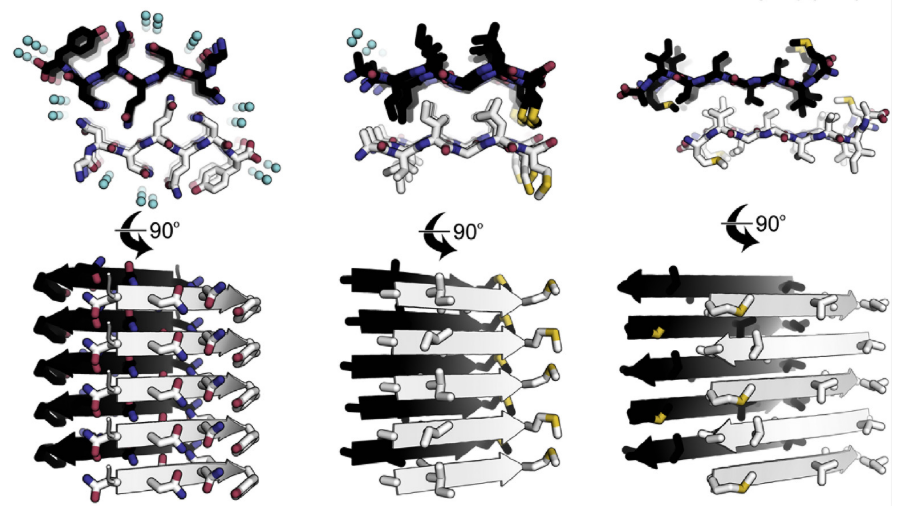
\includegraphics[scale=0.5]{amy.png}
    \label{fig:amy}
    \caption{Structure of amyloids showing possible configurations.}
\end{figure}

The following are important properties of amyloids that have been shown through experimentation \cite{Greenwald2018}:
1) they can be formed from simple sequences of short peptides;
2) they are more stable than isolated peptides;
3) they can catalyze reactions;
4) they can act as templates of their own replication;
5) they can interact with RNA, DNA, and polysaccharides.

The first and second properties possibly indicate that due to the simple and easy formation, there could be more amyloid peptides than sophisticated protein chains.
The catalysis of reactions is important in establishing simple metabolic pathways by interacting with DNA, RNA, and polysaccharides (sugars).
Finally, the ability to act as templates of their own replication may have also given cells the ability to reproduce.
These properties of amyloids can be related to the functional definition of life, in that it is able to carry out metabolic reactions and that it can reproduce amyloids (and as a possible consequence, genetic material).

%% something about the evolution of organic and other material
%% 9 requirements -- should probs follow
\subsection{Proposed requirements for the origin of life}
%% in here just detail the things
\citeA{Maruyama2019} propose the following requirements for the origin of life:

\begin{itemize}
    \item a reliable energy source;
    \item a supply of nutrients and elements found in living systems;
    \item high concentration of reduced gases;
    \item dry-wet cycles;
    \item non-toxic aqueous environment;
    \item ``cyclic conditions''
\end{itemize}

The proponents stated that some studies refute the possibility of the reduced atmosphere because they did not agree with the numerical calculations for the early atmosphere of the Earth.
However, they did not disagree with the fact taht organic molecules have come from the reduced gases.
If the reduced gases were not found in the atmosphere, a possibility is that the gases are dissolved.
Furthurmore, they have asserted that the only reasonable place for the origin of life is from the vicinity of natural nuclear reactors.
One of such has been found in Africa.
The theory is similar to the bubble hypothesis in a way that organic molecules have their origins in the sea.

The possibility of panspermia based on the proposed requirements cannot be falsified and hence may be dismissed until further factors are known \cite{Maruyama2019}.
The study is important since they have proposed necessary requirements for the possible origin of life.
This creates a scaffolding for future arguments on the topic.

\section{Cell origin}
%% use the one with the proposition that the protocell was 
%% without the membrane
The origin of the living cell is a complex phenomenon.
There are numerous theories in its development, such as the development of the membrane first before the necessary cellular faculties \cite{Matveev2019}.
In this section, the development of the primitive cell environment (the protocell) without the cellular phospholipid bilayer is discussed.
Biophysical arguments will primarily come from the hypothesis of \citeA{Matveev2019} on the development of the protocell.
Along with it, the general properties of life \cite[p.15]{biomain} will be used to strengthen the hypothesis.

\citeA{Matveev2019} defines the protocell the precursor of the cell.
Experiments have shown that the interior of the biological cell (the cytoplasm) has a different liquid ``phase'' relative to bulk water \footnote{regular liquid water}.
A difference in phase was explained to be the difference in the dissolving power of water in and out of the cell.
This observation was caused by the adsorption of water into hydrophilic groups of proteins in strong hydrogen bonds, increasing the energy required to dissolve substances.
Though this phenomenon is not observed in all proteins with hydrophilic groups, \citeA{Matveev2019} proposed that to ensure water adhesion, the substrate protein should have pockets with fixed charges where water can accumulate.
It was however noted that the energy difference is only slight compared to the bonding in bulk water, it was sufficient to reduce solubility!

The model of the protocell is capable of producing concentration gradients by pushing aqueous particles into and from different phases.
This can be though of as primitive homeostatic regulation and adaption.
It can also be thought of as cell growth through material exchange with the outside environment.
The model also can split into two in response to chemical cues in the environment which possibly a primitive form of reproduction.

Finally, from the development of the protocell with the important properties of life, the phase can be enclosed in the fluid mosaic phospholipid bilayer membrane through possible self-organization with present phospholipids in the aqueous environment forming \emph{the cell}.
